\documentclass[12pt]{article}
\usepackage[margin=2.5cm]{geometry}
\usepackage{enumerate}
\usepackage{amsfonts}
\usepackage{amsmath}
\usepackage{fancyhdr}
\usepackage{amsmath}
\usepackage{amssymb}
\usepackage{amsthm}
\usepackage{mdframed}
\usepackage{graphicx}
\usepackage{subcaption}
\usepackage{adjustbox}
\usepackage{listings}
\usepackage{xcolor}
\usepackage{booktabs}
\usepackage[utf]{kotex}
\usepackage{hyperref}

\definecolor{codegreen}{rgb}{0,0.6,0}
\definecolor{codegray}{rgb}{0.5,0.5,0.5}
\definecolor{codepurple}{rgb}{0.58,0,0.82}
\definecolor{backcolour}{rgb}{0.95,0.95,0.92}

\lstdefinestyle{mystyle}{
    backgroundcolor=\color{backcolour},
    commentstyle=\color{codegreen},
    keywordstyle=\color{magenta},
    numberstyle=\tiny\color{codegray},
    stringstyle=\color{codepurple},
    basicstyle=\ttfamily\footnotesize,
    breakatwhitespace=false,
    breaklines=true,
    captionpos=b,
    keepspaces=true,
    numbers=left,
    numbersep=5pt,
    showspaces=false,
    showstringspaces=false,
    showtabs=false,
    tabsize=1
}

\lstset{style=mystyle}

\pagestyle{fancy}
\renewcommand{\headrulewidth}{0.4pt}
\lhead{CSC 373}
\rhead{Worksheet 0 Solution}

\begin{document}
\title{CSC373 Worksheet 0 Solution}
\maketitle

\bigskip

\begin{enumerate}[1.]
    \item

    \underline{Recurrence:} $T(n) = T(n-1) + n$

    \bigskip

    \underline{Guess:} $T(n) = \mathcal{O}(n^2)$.

    \bigskip

    I need to show $T(n) \leq c \cdot n^2$.

    \bigskip

    \begin{align}
        T(n) &\leq c(n-1)^2 + n\\
        &= c(n^2 -2n + 1) + n\\
        &= cn^2 - c2n + c + n\\
        &\leq cn^2 - c2n + cn + n\\
        &= cn^2 - cn + n\\
        &\leq cn^2 - cn + cn\\
        &= cn^2
    \end{align}

    \bigskip

    \underline{\textbf{Notes:}}

    \bigskip

    \begin{itemize}
        \item Substitution method

        \begin{itemize}
            \item Solves recurrences
            \begin{itemize}
                \item Recurrence characters the running time of divide-and-conquer algorithm
            \end{itemize}
            \item How it works:

            \begin{enumerate}[1.]
                \item Make a guess for the solution
                \item Use mathematical induction to prove the guess is correct or incorrect.
            \end{enumerate}

            \bigskip

            \underline{\textbf{Example:}}

            \bigskip

            \underline{Recurrence:} $T(n) = 2T(\lfloor n/2 \rfloor) + n$

            \bigskip

            \underline{Guess:} $T(n) = \mathcal{O}(n\log n)$,

            \bigskip

            We need to show $T(n) \leq cn \lg n$.

            \bigskip

            \begin{enumerate}[1.]
                \item Assume the bound holds for all positive $m < n$, in particular $m = \lfloor n/2 \rfloor$
                \item Find the upper bound of $T(m)$

                \bigskip

                $T(\lfloor n/2 \rfloor) \leq c \lfloor n/2 \rfloor \lg (\lfloor n/2 \rfloor)$

                \bigskip

                \item Show $T(n) = 2T(\lfloor n/2 \rfloor) + n$ leads to $T(n) \leq cn \lg n$

                \bigskip

                \begin{align}
                    T(n) &\leq 2(c \lfloor n/2 \rfloor \lg (\lfloor n/2 \rfloor)) + n\\
                    &\leq cn \lg (n/2) + n\\
                    &= cn \lg (n) - cn \lg 2 + n\\
                    &= cn \lg (n) - cn + n\\
                    &\leq cn \lg (n) - cn + cn\\
                    &\leq cn \lg (n)
                \end{align}

                \item Show that the boundary holds using mathematical induction

                \bigskip

                \color{red}Doesn't have information in detail. Skipping this for now.\color{black}
            \end{enumerate}

            \item Making good guess

            \begin{itemize}
                \item Three suggestions
                \begin{enumerate}[1.]
                    \item Using recursion tree
                    \item Through practice
                    \item prove loose upper and lower bounds on the recurrence and then reduce the range of uncertainty
                \end{enumerate}
            \end{itemize}
        \end{itemize}
    \end{itemize}

    \item
    \setcounter{equation}{0}
    \underline{Recurrence:} $T(n) = T(\lceil n/2 \rceil) + 1$

    \bigskip

    \underline{Guess:} $T(n) = \mathcal{O}(\lg n)$.

    \bigskip

    I need to show $T(n) \leq c \cdot \lg n$.

    \bigskip

    \begin{align}
        T(n) &\leq c\lg (\lceil n/2 \rceil) + 1\\
        &\leq c \lg (n/2) + 1 \\
        &= c (\lg n - \lg 2) + 1\\
        &= c (\lg n - 1) + 1\\
        &= c\lg n - c + 1\\
        &\leq c\lg n - c + c
    \end{align}

    \bigskip

    \begin{mdframed}
        \setcounter{equation}{0}
        \underline{\textbf{Correct Solution:}}

        \bigskip

        \underline{Recurrence:} $T(n) = T(\lceil n/2 \rceil) + 1$

        \bigskip

        \underline{Guess:} $T(n) = \mathcal{O}(\lg n)$.

        \bigskip

        I need to show $T(n) \leq c \cdot \lg n$.

        \bigskip

        \begin{align}
            T(n) &\leq c\lg (\lceil n/2 \rceil) + 1\\
            &\leq c \lg (n/2) + 1 \\
            &= c (\lg n - \lg 2) + 1\\
            &= c (\lg n - 1) + 1\\
            &= c\lg n - c + 1\\
            &\leq c\lg n - c + c
        \end{align}

        \bigskip

        \color{red}The solution holds for $c \geq 1$.\color{black}

    \end{mdframed}

    \item
    \setcounter{equation}{0}
    \bigskip

    \underline{Recurrence:} $T(n) = 2T(\lfloor n/2 \rfloor) + n$

    \bigskip

    \underline{Guess (Upperbound):} $T(n) = \mathcal{O}(n\lg n)$.

    \bigskip

    I first need to show $T(n) \leq c \cdot n \lg n$.

    \bigskip

    \begin{align}
        T(n) &= 2T(\lfloor n/2 \rfloor) + n\\
        &= 2 c \lfloor n/2 \rfloor \lg \lfloor n/2 \rfloor + n\\
        &\leq 2 c \cdot (n/2) \lg (n/2) + n\\
        &= c \cdot n (\lg n - 1) + n\\
        &= cn \lg n - cn + n\\
        &\leq cn \lg n - cn + cn\\
        &\leq cn \lg n
    \end{align}

    \bigskip

    The above inequality holds for $c \geq 1$.

    \bigskip

    \underline{Guess (Lowerbound):} $T(n) = \Omega(n\lg n)$.

    \bigskip

    I first need to show $ d \cdot (n-2) \lg (n-2) \leq T(n)$.

    \bigskip

    \begin{align}
        T(n) &= 2T(\lfloor (n-2)/2 \rfloor) + n\\
        &\geq 2 d \lfloor (n-2)/2 \rfloor \lg \lfloor (n-2)/2 \rfloor + n\\
        &\geq 2 d \cdot ((n-2)/2) \lg ((n-2)/2) + n\\
        &= d \cdot (n-2) (\lg (n-2) - 1) + n\\
        &= d \cdot (n - 2) \lg (n - 2) - d \cdot (n - 2) + n\\
        &\geq d \cdot (n - 2) \lg (n - 2) - d \cdot (n - 2) + (n-2)\\
        &\geq d \cdot (n - 2) \lg (n - 2) - d \cdot (n - 2) + d \cdot (n-2)\\
        &= d \cdot (n - 2) \lg (n - 2)
    \end{align}

    \bigskip

    The above inequality holds for $0 \leq d < 1$.

    \bigskip

    \underline{\textbf{Notes:}}

    \bigskip

    \begin{itemize}
        \item Both upper bound and lower bound don't need to be the same

        \begin{center}
        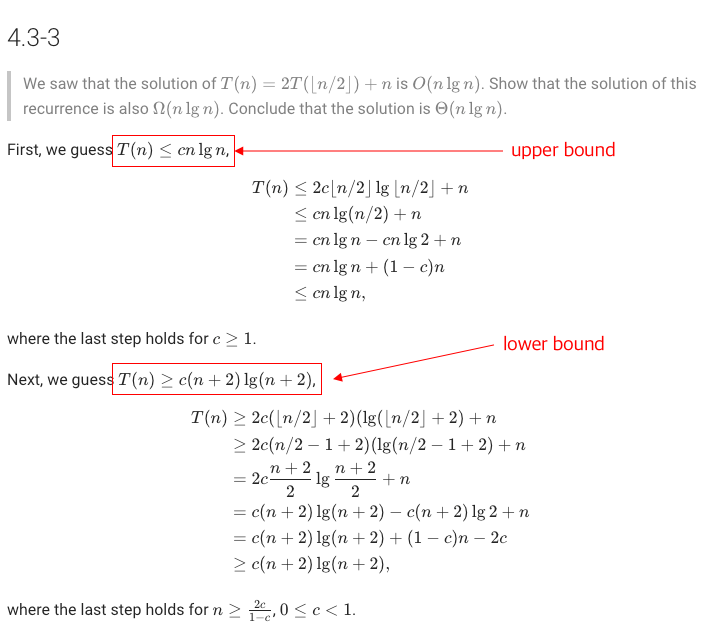
\includegraphics[width=0.7\linewidth]{images/worksheet_0_solution_1.png}
        \end{center}
    \end{itemize}

    \item
    \setcounter{equation}{0}
    \underline{Recurrence (Merge sort):}

    \begin{align*}
        T(n) =
        \begin{cases}
          \Theta(1) & \text{if $n = 1$}\\
          T(\lceil n/2 \rceil) + T(\lfloor n/2 \rfloor) + \Theta(n) & \text{if $n > 1$}
        \end{cases}
    \end{align*}

    \bigskip

    \underline{Guess (upper bound):} $T(n) \leq c \cdot (n-2) \cdot \lg (n-2)$

    \bigskip

    \begin{align}
        T(n) &\leq c(\lceil n/2 \rceil - 2) \lg (\lceil n/2 \rceil - 2) + c (\lfloor n/2 \rfloor - 2)\lg(\lfloor n/2 \rfloor - 2) + dn\\
        &= c(n/2 + 1 - 2) \lg (n/2 + 1 - 2) + c (n/2 + 1 - 2)\lg(n/2 + 1 - 2) + dn\\
        &= c((n-2)/2) \lg ((n-2)/2) + c ((n-2)/2)\lg((n-2)/2) + dn\\
        &= c(n-2) \lg ((n-2)/2) + dn\\
        &= c(n-2) \lg (n-2) - c(n-2) + dn\\
        &= c(n-2) \lg (n-2) - (d - c)n + 2c\\
        &= c(n-2) \lg (n-2)
    \end{align}

    \bigskip

    The bound holds as long as $c > d$.

    \bigskip

    \underline{Guess (lower bound):} $c \cdot (n-2) \cdot \lg (n-2) \leq T(n)$


    \bigskip

    \begin{align}
        T(n) &\leq c(\lceil n/2 \rceil + 1) \lg (\lceil n/2 \rceil + 1) + c (\lfloor n/2 \rfloor + 1)\lg(\lfloor n/2 \rfloor + 1) + dn\\
        &\leq c(n/2 - 1 + 1) \lg (n/2 - 1 + 1) + c (n/2 - 1 + 1)\lg(n/2 - 1 + 1) + dn\\
        &= c(n/2) \lg (n/2) + c (n/2)\lg(n/2) + dn\\
        &= cn \lg(n/2) + dn\\
        &= cn \lg(n) - cn + dn\\
        &= cn \lg(n) + (d - c)n\\
        &\leq c(n-1) \lg(n-1)
    \end{align}

    \bigskip

    The bound holds as long as $d > c$, and $0 \leq c < 1$

    \bigskip


    \underline{\textbf{Notes:}}

    \bigskip

    \begin{itemize}
        \item the $n$ here is asymptotically large
    \end{itemize}

\end{enumerate}

\end{document}